\newpage
\subsection{Frequenzmessung}\label{sec:2-3}
\subsubsection{Aufgabenstellung}

Mit einer Wien Robinson Brücke sollen zwei verschiedene Frequenzen gemessen werden. Dabei werden $f_1 = \SI{1}{\kilo\hertz}$ und $f_2 = \SI{5}{\kilo\hertz}$ gewählt. Mit dem Oszilloskop müssen die Frequenzen nachgeprüft werden.

\subsubsection{Verwendetes Material}

\begin{table}[h]
	\centering
	\caption{Verwendetes Material}
	\begin{tabularx}{\textwidth}{XXX}
		\textbf{Material}  & \textbf{Verwendung}        & \textbf{Anmerkungen}           \\ \midrule
		RL-Blackbox        & Messobjekt ($L_1 + R_1$)   &                                \\
		2x C-dekade        & Abgleich Kondensator ($C$) &                                \\
		RS-200             & Abgleichwiderstand ($R_1$) & $\pm (1\% + \SI{0.025}{\ohm})$ \\
		R-DIG-6            & Abgleichwiderstand ($R_2$) & $\pm (1\% + \SI{0.025}{\ohm})$ \\
		Funktionsgenerator & Hilfsspannung ($U_H$)      & $V_{PP} = \SI{10}{\volt}$      \\
		Oszilloskop        & Nullinstrument ($NI$)      &                                \\
	\end{tabularx}
\end{table}

\subsubsection{Versuchsaufbau}

Die Frequenz ist mit der Fequenzbrücke von Wien-Robinson~\hyperref[fig:Fequenzbruecke-Wien-Robinson]{(Abb.~\ref{fig:Fequenzbruecke-Wien-Robinson})} zu bestimmen. Wobei $R_3=\SI{22}{\kilo\ohm}$, $R_4=\SI{10}{\kilo\ohm}$ und $C = \SI{0.1}{\mu\farad}$ fixiert wurde.

\begin{figure}[h]
	\begin{center}
		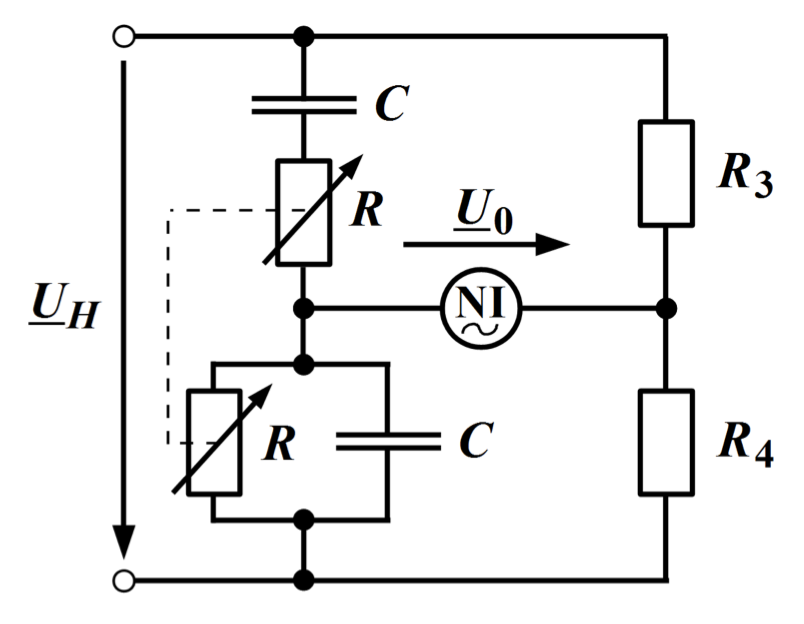
\includegraphics[width=0.45\textwidth]{images/Fequenzbruecke-Wien-Robinson.png}
	\end{center}
	\caption{Fequenzbruecke nach Wien-Robinson}\label{fig:Fequenzbruecke-Wien-Robinson}
\end{figure}

\subsubsection{Herleitung Abgleichbedingung}

\begin{align}
	\left(R + \frac{1}{j\omega C}\right) R_4
	 & = \frac{R\,\frac{1}{j\omega C}}{R + \frac{1}{j\omega C}}\, R_3
\end{align}

\begin{align}
	R^2 R_4 - \frac{R_4}{\omega^2 C^2} - j\,\frac{2 R R_4}{\omega C}
	 & = -\, j\, \frac{R R_3}{\omega C}
\end{align}

\begin{align}
	\omega & = \frac{1}{R C} \\
	R_3    & = 2 R_4
\end{align}

\begin{align}
	f & = \frac{1}{2\pi R C}
\end{align}
% subsection Herleitung Abgleichbedingung (end)

\subsubsection{Abgleich mit Oszilloskop}
Für $f_1=\SI{1}{\kilo\hertz}$:
\begin{gather}
	R=\SI{1590}{\ohm} \\
	f_{1,\text{mess}}=\tfrac{1}{2\pi \cdot \SI{159}{\ohm} \cdot \SI{0.1}{\mu\farad}} = \SI{1000,97}{\hertz}
\end{gather}
Für $f_2=\SI{5}{\kilo\hertz}$:
\begin{gather}
	R=\SI{318}{\ohm} \\
	f_{2,\text{mess}}=\tfrac{1}{2\pi \cdot \SI{318}{\ohm} \cdot \SI{0.1}{\mu\farad}} = \SI{5004.87}{\hertz}
\end{gather}

\begin{figure}[h]
	\begin{minipage}[position]{0.48\textwidth}
		\centering
		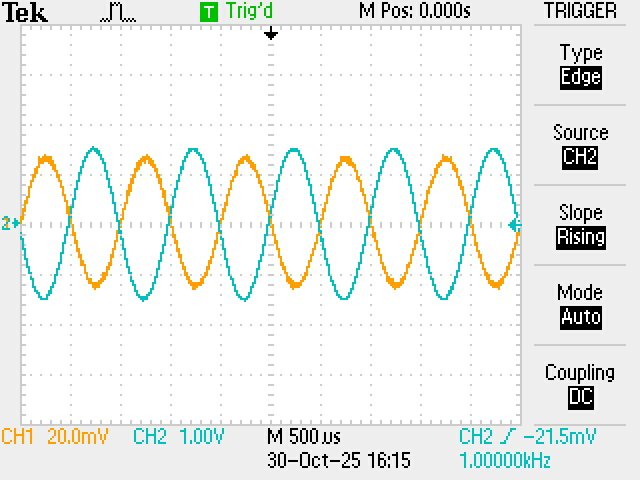
\includegraphics[height=4.5cm]{images/Abgleich-Frequenzmessung1.JPG}
		\caption{$f_1=\SI{1}{\kilo\hertz}$}
	\end{minipage}\hfill
	\begin{minipage}[position]{0.48\textwidth}
		\centering
		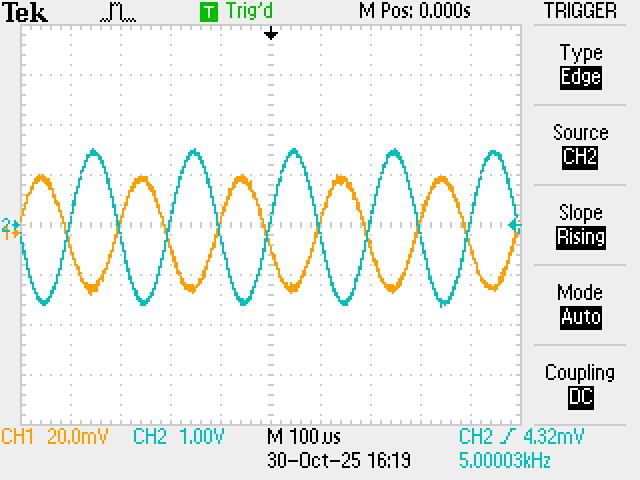
\includegraphics[height=4.5cm]{images/Abgleich-Frequenzmessung2.JPG}
		\caption{$f_2=\SI{5}{\kilo\hertz}$}
	\end{minipage}
\end{figure}



\subsubsection{Erkenntnisse}
Die Messungen stimmen erstaunlich gut mit den wahren Frequenzen überein. Das ist überraschend, da aufgrund der beschränkten Einstellbarkeit der Potentiometer fuer $R_3=\SI{22}{\kilo\ohm}$ und $R_4=\SI{10}{\kilo\ohm}$ deren Verhältnis $2.2:1$ statt $2:1$ ist. Das deutet darauf hin das ein genauer Ableich nicht möglich sein sollte.

